\documentclass{article}
\title{Zadanie 6 - projekt własny}
\author{Dominik Kuczkowski 180235\\
Izabela Załęska 180322}
\date{06.06.2022}

\usepackage[T1]{fontenc}
\usepackage{graphicx}
\usepackage{geometry}
\geometry{
    a4paper,
    total={170mm,257mm}
}
\usepackage{listings}

\begin{document}
\maketitle
\newpage
\section{Założenia}
\begin{itemize}
    \item Aplikacja będzie służyć do prostej wizualicaji 2D robota przemysłowego
    \item Aplikacja posiadać będzie interfejs graficzny
    \item Możliwe będzie zapisywanie ruchów robota
    \item Robot wyposażony będzie w magnes, który umożliwi mu przenoszenie klocków z miejsca na miejsce
    \item Możliwe będzie sterowanie robotem za pomocą klawiatury
    \item Program napisany zostanie w języku C++ z wykorzystaniem biblioteki SFML
\end{itemize}
\section{Opis programu}
\subsection{Interfejs graficzny}
\begin{figure}[h!]
    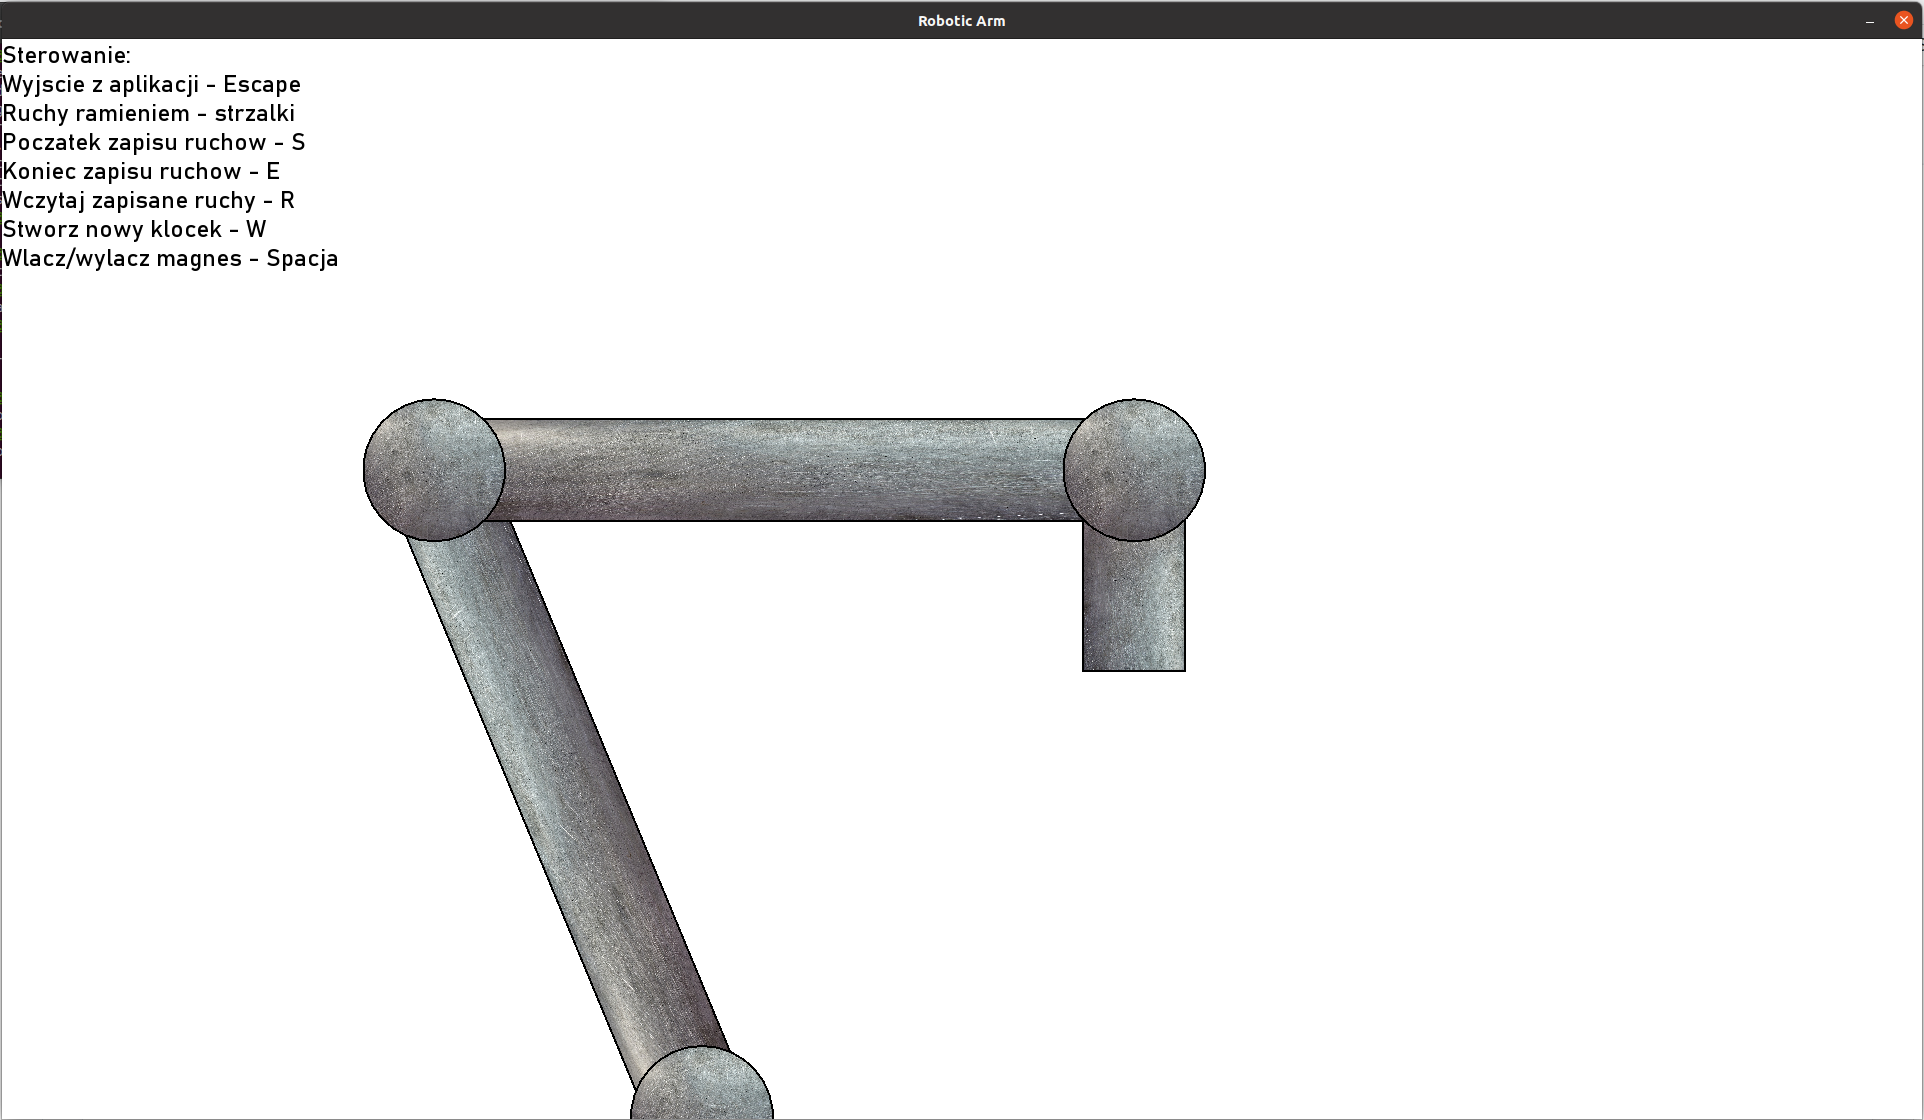
\includegraphics[width=\linewidth]{RoboticArm.png}
    \caption{Interfejs graficzny}
    \label{intgraf}
\end{figure}
Na rys. \ref{intgraf} przedstawiony został interfejs graficzny
programu. Przedstawia on prostą wizualizację ramienia robotycznego o 
trzech jointach. W oknie programu wyświetlany jest sposób sterowania robotem.
Wykorzystuje się do tego strzałki. Klawisz W umożliwia stworzenie klocka, 
który pojawia się u dołu ekranu. Wciśnięcie spacji włącza lub wyłącza magnes
na końcu ostatniego z fragmentów robota. Umożliwia to przenoszenie klocków.
Klawisze S, E i R służą do zapisu i odtwarzania ruchów robota.
\subsection{Implementacja}
Punktem startowym programu jest plik main.cpp, w którym odbywa się
stworzenie instancji klasy robot oraz uruchamiana jest pętla programu.
W pętli wywoływane są metody update() i render() z klasy Robot. Metoda update
odpowiada za wywoływanie wewnętrznych metod związanych z obsługą klawiatury i 
zmianą stanu programu. Metoda render wywołuje funkcje związane z wyświetlaniem
obrazu. W programie do odczytywania klawiszy z klawiatury wykorzystywane są
Eventy udostępniane przez bibliotekę SFML. 
\begin{figure}[h!]
    \includegraphics[width=\linewidth]{events.png}
    \caption{Funkcja czytająca klawisze}
    \label{events}
\end{figure}
Na rys. \ref{events} przedstawiona jest funkcja sprawdzająca wciśnięcie klawiszy
odpowiedzialnych za zamykanie okna, tworzenie klocków oraz włączanie magnesu.
\newpage
Jak widać biblioteka udostępnia przyjemne API do sprawdzania zarówno czy klawisz 
został wciśnięty czy puszczony. Po sprawdzeniu klawiszy w programie 
wywoływana jest funkcja poruszająca ramieniem, która reaguje na eventy od strzałek.
\begin{figure}[h!]
    \includegraphics[width=\linewidth]{arm.png}
    \caption{Funkcja obliczająca nowe położenia przegubów robota}
    \label{arm}
\end{figure}
Wyliczanie nowych pozycji poszczególnych elementów robota odbywa się za pomocą 
funkcji trygonometrycznych, co zostało przedstawione na rys. \ref{arm}.
\newpage
W programie zaimplementowano opcję zapisu ruchów robota. Odbywa się ona z wykorzystaniem
strutktury danych z biblioteki standardowej - Queue.
\begin{figure}[h!]
    \includegraphics[width=\linewidth]{queue.png}
    \caption{Dodawanie do kolejki jednego z ruchów robota}
    \label{queue}
\end{figure}
Na rys. \ref{queue} pokazany jest moment zapisu do kolejki jednego z ruchów robota.
Zapisywany jest numer przegubu, który wykonuje ruch oraz kąt o jaki należy ten przegub 
przesunąć. Taki sposób zapisu pozwala w łatwy sposób wczytywać ruchy.
\section{Omówienie wyników}
Program spełnia swoje założenia co do symulowania prostych ruchów robota na płaszczyźnie.
Wadą projektu jest bardzo prosta symulacja, która pozwala na łapanie tylko kwadratowych przedmiotów.
Zaletą projektu jest dobrze napisany kod w C++, który działa wydajnie i mógłby zostać z powodzeniem
rozszerzony o nowe funkcjonalności.
\end{document}